%%%%%%%%%%%%%%%%%%%%%%%%%%%%%%%%%%%%%%%%%
% Arsclassica Article
% LaTeX Template
% Version 1.0 (21/4/14)
%
% This template has been downloaded from:
% http://www.LaTeXTemplates.com
%
% Original author:
% Lorenzo Pantieri (http://www.lorenzopantieri.net) with extensive modifications by:
% Vel (vel@latextemplates.com)
%
% License:
% CC BY-NC-SA 3.0 (http://creativecommons.org/licenses/by-nc-sa/3.0/)
%
%%%%%%%%%%%%%%%%%%%%%%%%%%%%%%%%%%%%%%%%%

%----------------------------------------------------------------------------------------
%	PACKAGES AND OTHER DOCUMENT CONFIGURATIONS
%----------------------------------------------------------------------------------------

\documentclass[
10pt, % Main document font size
a4paper, % Paper type, use 'letterpaper' for US Letter paper
oneside, % One page layout (no page indentation)
%twoside, % Two page layout (page indentation for binding and different headers)
headinclude,footinclude, % Extra spacing for the header and footer
BCOR5mm, % Binding correction
]{scrartcl}

%%%%%%%%%%%%%%%%%%%%%%%%%%%%%%%%%%%%%%%%%
% Arsclassica Article
% Structure Specification File
%
% This file has been downloaded from:
% http://www.LaTeXTemplates.com
%
% Original author:
% Lorenzo Pantieri (http://www.lorenzopantieri.net) with extensive modifications by:
% Vel (vel@latextemplates.com)
%
% License:
% CC BY-NC-SA 3.0 (http://creativecommons.org/licenses/by-nc-sa/3.0/)
%
%%%%%%%%%%%%%%%%%%%%%%%%%%%%%%%%%%%%%%%%%

%----------------------------------------------------------------------------------------
%	REQUIRED PACKAGES
%----------------------------------------------------------------------------------------

\usepackage[
nochapters, % Turn off chapters since this is an article        
beramono, % Use the Bera Mono font for monospaced text (\texttt)
eulermath,% Use the Euler font for mathematics
pdfspacing, % Makes use of pdftex’ letter spacing capabilities via the microtype package
dottedtoc % Dotted lines leading to the page numbers in the table of contents
]{classicthesis} % The layout is based on the Classic Thesis style

\usepackage{arsclassica} % Modifies the Classic Thesis package

\usepackage[T1]{fontenc} % Use 8-bit encoding that has 256 glyphs

\usepackage[utf8]{inputenc} % Required for including letters with accents

\usepackage{graphicx} % Required for including images
\graphicspath{{Figures/}} % Set the default folder for images

\usepackage{enumitem} % Required for manipulating the whitespace between and within lists

\usepackage{lipsum} % Used for inserting dummy 'Lorem ipsum' text into the template

\usepackage{subfig} % Required for creating figures with multiple parts (subfigures)

\usepackage{amsmath,amssymb,amsthm} % For including math equations, theorems, symbols, etc

\usepackage{varioref} % More descriptive referencing

\usepackage{hyperref}

\usepackage{float}

%----------------------------------------------------------------------------------------
%	THEOREM STYLES
%---------------------------------------------------------------------------------------

\theoremstyle{definition} % Define theorem styles here based on the definition style (used for definitions and examples)
\newtheorem{definition}{Definition}

\theoremstyle{plain} % Define theorem styles here based on the plain style (used for theorems, lemmas, propositions)
\newtheorem{theorem}{Theorem}

\theoremstyle{remark} % Define theorem styles here based on the remark style (used for remarks and notes)

%----------------------------------------------------------------------------------------
%	HYPERLINKS
%---------------------------------------------------------------------------------------

\hypersetup{
%draft, % Uncomment to remove all links (useful for printing in black and white)
colorlinks=true, breaklinks=true, bookmarks=true,bookmarksnumbered,
urlcolor=webbrown, linkcolor=RoyalBlue, citecolor=webgreen, % Link colors
pdftitle={Orsay Museum}, % PDF title
pdfauthor={\textcopyright}, % PDF Author
pdfsubject={Orsay Museum}, % PDF Subject
pdfkeywords={Orsay, Orsay Museum, Musee d'Orsay, Museum, Emre Ozan Alkan}, % PDF Keywords
pdfcreator={pdfLaTeX}, % PDF Creator
pdfproducer={LaTeX with hyperref and ClassicThesis} % PDF producer
}

\hyphenation{Fortran hy-phen-ation} % Specify custom hyphenation points in words with dashes where you would like hyphenation to occur, or alternatively, don't put any dashes in a word to stop hyphenation altogether

%----------------------------------------------------------------------------------------
%	TITLE PAGE
%----------------------------------------------------------------------------------------
\newcommand*{\titleGM}{\begingroup % Create the command for including the title page in the document
\hbox{ % Horizontal box
\hspace*{0.2\textwidth} % Whitespace to the left of the title page
\rule{1pt}{\textheight} % Vertical line
\hspace*{0.05\textwidth} % Whitespace between the vertical line and title page text
\parbox[b]{0.75\textwidth}{ % Paragraph box which restricts text to less than the width of the page

{\noindent\Huge\bfseries Musée \\[0.5\baselineskip] d'Orsay}\\[2\baselineskip] % Title
{\large \textit{Local Culture Survey}}\\[4\baselineskip] % Tagline or further description
{\Large \textsc{Emre Ozan Alkan}} % Author name

\vspace{0.5\textheight} % Whitespace between the title block and the publisher
%{\noindent The Publisher \plogo}
\today
%\\[\baselineskip] % Publisher and logo
}}
\endgroup}

%----------------------------------------------------------------------------------------
%	TITLE AND AUTHOR(S)
%----------------------------------------------------------------------------------------

\title{\normalfont\spacedallcaps{Musée d'Orsay}} % The article title

\author{\spacedlowsmallcaps{Emre Ozan Alkan\textsuperscript{1}}} % The article author(s) - author affiliations need to be specified in the AUTHOR AFFILIATIONS block

\date{\today} % An optional date to appear under the author(s)

%----------------------------------------------------------------------------------------

\begin{document}

\titleGM % This command includes the title page

%----------------------------------------------------------------------------------------
%	HEADERS
%----------------------------------------------------------------------------------------

\renewcommand{\sectionmark}[1]{\markright{\spacedlowsmallcaps{#1}}} % The header for all pages (oneside) or for even pages (twoside)
%\renewcommand{\subsectionmark}[1]{\markright{\thesubsection~#1}} % Uncomment when using the twoside option - this modifies the header on odd pages
\lehead{\mbox{\llap{\small\thepage\kern1em\color{halfgray} \vline}\color{halfgray}\hspace{0.5em}\rightmark\hfil}} % The header style

\pagestyle{scrheadings} % Enable the headers specified in this block

%----------------------------------------------------------------------------------------
%	TABLE OF CONTENTS & LISTS OF FIGURES AND TABLES
%----------------------------------------------------------------------------------------

\pagestyle{empty} % Removes page numbers
\clearpage
\setcounter{page}{2}

\maketitle % Print the title/author/date block

\setcounter{tocdepth}{1} % Set the depth of the table of contents to show sections and subsections only

\tableofcontents % Print the table of contents

\listoffigures % Print the list of figures

\listoftables % Print the list of tables

%\thispagestyle{empty}

%----------------------------------------------------------------------------------------
%	ABSTRACT
%----------------------------------------------------------------------------------------

\section*{Abstract} % This section will not appear in the table of contents due to the star (\section*)

%Attracting more than two million visitors a year, the Orsay Museum
%
%the Orsay Museum is a major destination for art lovers
 
Musée d'Orsay is a museum in Paris, on the left bank of the Seine River. Formerly it was Garde d'Orsay, a Beaux-Arts railway station completed in 1900. The museum holds mainly French art dating from 1845s to 1915s, including paintings, sculptures, furniture and photography. Attracting nearly three million visitors a year, It's a major destination for art lovers which known with largest collection of impressionist masterpieces in world. In this paper, a survey of the Orsay Museum is presented. The focus is on a general history of the museum, importance for impressionism and artworks exhibited in the museum.

%\lipsum[1] % Dummy text

%----------------------------------------------------------------------------------------
%	AUTHOR AFFILIATIONS
%----------------------------------------------------------------------------------------

\let\thefootnote\relax\footnotetext{\textsuperscript{1} \textit{Masters in Computer Vision, University of Burgundy, France}}

%\let\thefootnote\relax\footnotetext{* \textit{Department of Biology, University of Examples, London, United Kingdom}}

%\let\thefootnote\relax\footnotetext{\textsuperscript{1} \textit{Department of Chemistry, University of Examples, London, United Kingdom}}

%----------------------------------------------------------------------------------------

\newpage % Start the article content on the second page, remove this if you have a longer abstract that goes onto the second page

\pagestyle{scrheadings}

%----------------------------------------------------------------------------------------
%	INTRODUCTION
%----------------------------------------------------------------------------------------

\section{History of the Museum}

\paragraph{} Attracting nearly three million visitors a year, It's a major destination for art lovers which known with largest collection of impressionist masterpieces in world.

\paragraph{} It's history is quite interesting. The building was formerly a railway station known as Gare d'Orsay, built for early French railway company Chemin de Fer de Paris a Orleans. The building finished in 1900 for Exposition Universelle by three architects: Lucien Magne, Emile Benard and Cictor Laloux.

%A statement requiring citation \cite{Figueredo:2009dg}.

%\lipsum[1-3] % Dummy text

%Some mathematics in the text: $\cos\pi=-1$ and $\alpha$.

\subsection{The site}
\paragraph{}Musee d'Orsay's site has very old history.
\begin{quote}
The rue de Lille was once the central lane of the garden belonging to Henri IV's famous queen, Marguerite de Valois. On her death in 1615, the property was sold by lots, and private mansions continued to build up the neighbourhood, while on the banks of the Seine a port known as the Grenouillière served as a resting place for lumber barges and other cargo. The construction of the Quai d'Orsay began in 1708 near the Pont Royal, and was completed a century later under Napoleon I's Empire. The aristocratic vocation of the neighbourhood was already well established at the end of the 18th century, when the Hôtel de Salm (today the Musée de la Légion d'honneur) was built, between 1782 and 1788.
\cite{orsayMuseumHistory}
\end{quote}

\begin{figure}[tbh]
\centering

\subfloat[Palais d'Orsay]{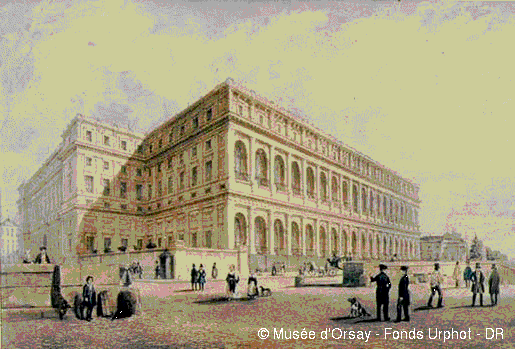
\includegraphics[width=.45\columnwidth]{Images/1.png}}
\label{fig:Palais}
 \quad
\subfloat[Démolition des ruines de la cour des comptes]{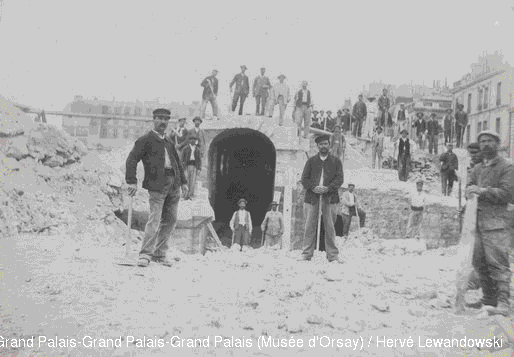
\includegraphics[width=.45\columnwidth]{Images/2.png}\label{fig:Demolition}}

\caption[Site pictures]{Site pictures from 19th century} % The text in the square bracket is the caption for the list of figures while the text in the curly brackets is the figure caption
\label{fig:Site}
\end{figure}

Before burnt due to violent Paris Commune action in 1871, two buildings are built on the site of Orsay station. First Cavalry barracks, and then the Palais d'Orsay is built between 1810 and 1838 by Jean-Charles Bonnard and Jacques Lacornee. 

\subsection{The Station}

\paragraph{}Before Exposition Universelle in 1900, French Orleans railroad company asked French government to take the land of ruined palaid d'Orsay. In that time the railroad company had far located station from center of the city, which was causing them disadvatages.

French government decided to give the land to the Orleans railroad company. In 1897, the company hired three architects: Lucien Magne, Emile Benard and Victor Laloux. The task of the architects were not because of the rich surrounding culture like Louvre and Palas de la Legion d'honneur. 

In July 14th, 1900, the station and hotel - built in two years - were opened. One of the architect Laloux, decided to mask the modern metallic structures with the facade of the hotel, that built in the academic style using finely cut stones from the regions of Charente and Poitou.

\begin{figure}[tbh]
\centering

\subfloat[La gare d'Orsay en cours de construction]{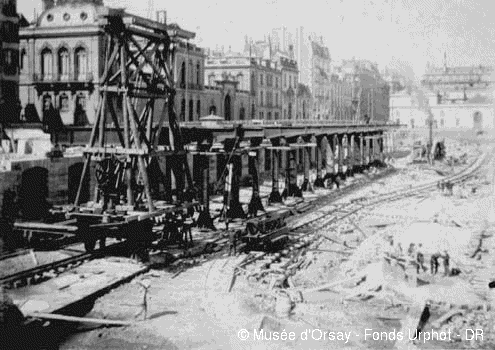
\includegraphics[width=.31\columnwidth]{Images/3.png}}\quad
\subfloat[Anonyme Sous le plancher métallique de]{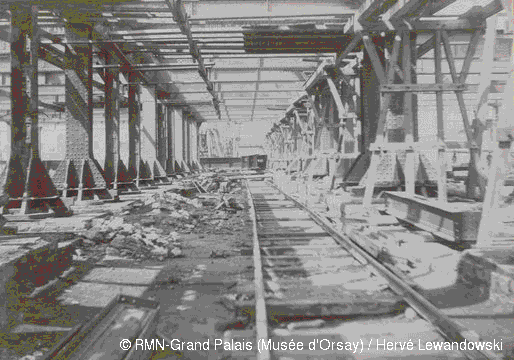
\includegraphics[width=.31\columnwidth]{Images/4.png}} \quad
\subfloat[The Gare d'Orsay]{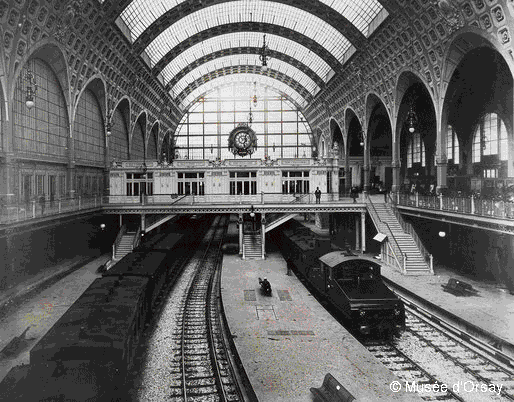
\includegraphics[width=.31\columnwidth]{Images/5.png}}

\caption[Pictures of the station]{Pictures of the station} % The text in the square bracket is the caption for the list of figures while the text in the curly brackets is the figure caption
\label{fig:station}
\end{figure}

Inside the building, all modern techniques are used, i.e., lifts for luggages, passenger elevators, ramps, sixteen underground railtracks and electric tractions. The open porch through the great hall was approximately 32 meters high, 40 meters wide and 138 meters long.

The Gare d'Orsay, till 1939s, was main railroad network of the southwestern French. It's hotel hosted many travelers, political party meetings, and famous people. Unfortunately, after 1939, the station became short for the modern and longer trains after electrification of the railroads. Later on station only served to suburbs. 

\subsection{Station to Museum}

\paragraph{}
Before serving as The Gare d'Orsay, the building used as many purposes, i.e, mailing center for sending packages, set for several films, haven. 

\begin{figure}[tbh]
\centering
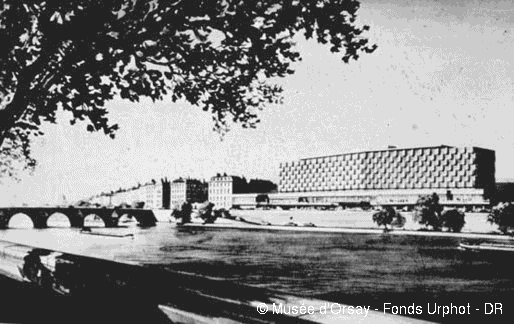
\includegraphics[width=.60\columnwidth]{Images/6.png}
\caption[Projet Guillaume Gillet-René Coulon]{Projet Guillaume Gillet-René Coulon} % The text in the square bracket is the caption for the list of figures while the text in the curly brackets is the figure caption
\label{fig:station2museum}
\end{figure}

In 1975, the Direction des Musées de France decided to build a new museum in the train station. They decided to present arts from the second half of the 19th century. In March 8, 1973, the station listed on the Supplementary Inventory of Historical Monuments. The official decision of building Musee d'Orsay appeared in October 20, 1977 by inter-ministerial council and President Valery Giscard d'Estaing's acts.

Then the building started to be know as a Historical Monument in 1978 and a civil commission was assembled to supervise the construction and organization of the museum. Fancois Mitterrand, the President of the republic, introduced the new museum on December 1st, 1985, and it opened to the public on December 9th.


\subsection{Architecture}

\begin{quote}
"The station is superb and looks like a Palais des beaux-arts..." wrote the painter Edouard Detaille in 1900. Eighty-six years later, his prophecy was fulfilled.\cite{orsayMuseumHistory}
\end{quote}

\paragraph{} The architectural change of the station into a museum was done by ACT architecture group, consist of M. Bardon, M. Colboc, and M. Philippon. Their project project proposal was approved in 1979 out of other six propositions. They respected Laloux's previous architecture with reinterpreting it due to new functionality. New architecture highlights its great hall using it as the main artery of the visit, and used impressively beautiful glass awning into the museum's entrance.

\begin{figure}[tbh]
\centering

\subfloat[Vue intérieure de la nef en travaux]{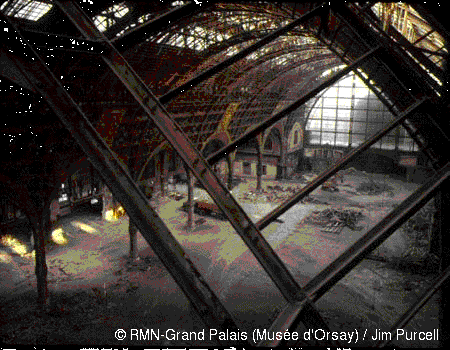
\includegraphics[width=.45\columnwidth]{Images/7.png}}
\label{fig:Palais}
 \quad
\subfloat[La salle du restaurant en travaux]{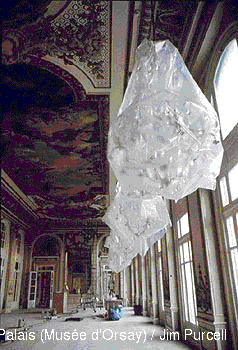
\includegraphics[width=.45\columnwidth]{Images/8.png}\label{fig:Demolition}}

\caption[Architecture pictures]{Architecture pictures} % The text in the square bracket is the caption for the list of figures while the text in the curly brackets is the figure caption
\label{fig:Architecture}
\end{figure}

Organization of the museum compose of three floor. First floor, the ground floor, many galleries are exhibited on either side of the central nave. Second floor, overlooks the first floor, opening up into additional exhibition galleries. The top floor is built above the lobby, which covers the lenghth of the Quai, and continues into the highest elevations of the former hotel, over the rue de la Legion d'Honneur. 

Not only the galleries but museum's specific exhibition spaces and different facilities are distributed throughout the three levels, i.e., the pavilion Amont, the glass walkway of the former station's western pinion, the museum restaurant, the Cafe des Hauterus, the bookshop and the auditorium.

\subsection{Facts}

Here are the some facts about Musee d'Orsay:\cite{orsayMuseumHistory}

\begin{table}[h]
\centering
\begin{tabular}{|c|c|l|l|l|}
\hline
\textbf{Year} & \multicolumn{4}{c|}{\textbf{Number of visitors}} \\ \hline
1994 and 2003 & \multicolumn{4}{c|}{2,239,050} \\ \hline
2004 & \multicolumn{4}{c|}{2,590,316} \\ \hline
2005 & \multicolumn{4}{c|}{2,929,282} \\ \hline
2006 & \multicolumn{4}{c|}{3,009,203} \\ \hline
2007 & \multicolumn{4}{c|}{3,166,509} \\ \hline
2008 & \multicolumn{4}{c|}{3,025,164} \\ \hline
2009 & \multicolumn{4}{c|}{3,022,012} \\ \hline
2010 & \multicolumn{4}{c|}{2,985,510} \\ \hline
2011 & \multicolumn{4}{c|}{3,144,449} \\ \hline
2012 & \multicolumn{4}{c|}{3,579,130} \\ \hline
\multicolumn{5}{|c|}{Total over 26 years: 74,453,766 visitors} \\ \hline
\end{tabular}
\caption{Annual frequentation of the museum}
\label{tab:numberVisitor}
\end{table}

\paragraph{}The Building
\begin{itemize}
	\item Length without the awning: 173 metres (189 yards, 567'7")
	\item Length including awning: 188 metres (205 $\frac{31}{2}$ yards, 616'9")
	\item Breadth: 75 metres (82 yards, 246')
\end{itemize}


\paragraph{}The Hall under the Nave
\begin{itemize}
	\item Length: 138 metres (150 $\frac{3}{4}$ yards, 452'9")
	\item Breadth: 40 metres (43 $\frac{3}{4}$ yards, 131')
	\item Height: 32 metres (104'11")
\end{itemize}

\paragraph{}The Materials
\begin{itemize}
	\item 12 000 metric tons of metallic structures
	\item 35 000 square metres of glass
	\item 1 600 staff rose casings in the nave
\end{itemize}

%\paragraph{}Annual number of visitors
%\begin{itemize}
%	\item 2,239,050 visitors in average per year between 1994 and 2003
%	\item 2,590,316 visitors in 2004
%	\item 2,929,282 in 2005
%	\item 3,009,203 in 2006
%	\item 3,166,509 in 2007
%	\item 3,025,164 in 2008
%	\item 3,022,012 in 2009
%	\item 2,985,510 in 2010
%	\item 3,144,449 in 2011
%	\item 3,579,130 in 2012
%\end{itemize}
%
%Total over 26 years
%74,453,766 visitors

\paragraph{}A Few Technical Data
\begin{itemize}
	\item 1 million cubic metres of air treated each hour for air conditioning
	\item 40,000 acoustic resonators
	\item 7,500 kWh of installed electric power
	\item 2 generating sets
	\item 10 escalators
	\item 12 elevators and lifts
\end{itemize}

%One of the world's most-visited museum, it houses largest collection of painting, sculpture and decorative objects.

%The museum contained more than 2300 paintings, 1500 sculptures, and 1000 other objects. 

%Opening times: 09.30 AM - 06.30 PM on Tuesday, Wednesday, Friday, Saturday and Sunday. 09.30 AM - 09.45 PM on Thursday. Monday closed.



 
%----------------------------------------------------------------------------------------
%	METHODS
%----------------------------------------------------------------------------------------

\section{Importance for Impressionism}

\subsection{What is impressionism ? }

\paragraph{}
It's a 19th century artistic movement based on a group of Paris-based artists. They reject the rules of academic painting. Their paintings has lots of color as well as very bright and vibrant and they are mostly outdoor scenes. Using primary colors and short brushstrokes to represent the appearance of reflected light, desired result of impressionism was to capture the artist's perception of the subject rather than the subject itself. 


\subsection{Orsay's importance}

\begin{quote}
“…the exhibition pays homage to French genius, that of Impressionism and that of the savoir-faire of the 19th century.” Guy Courgeval, curator, Musée d’Orsay.
\end{quote}

\begin{quote}
"The great Gallery of Impressionists should be rethought. There are there many masterpieces, but the addition of such a number of paintings of similar dimensions is prejudicial to visitor's vision", Mr Serge Lemoine, "Express Magazine" (in june 2002).
\end{quote}


\paragraph{}

One of the world's most-visited museum, it houses largest collection of painting, sculpture and decorative objects produced between 1848-1914. 

The Musee d'Orsay's collection of impressionist and post-impressionist paintings give taste of the finest experience of its kind in the world.

%Reference to Figure~\vref{fig:gallery}. % The \vref command specifies the location of the reference

%\begin{figure}[tbh]
%\centering 
%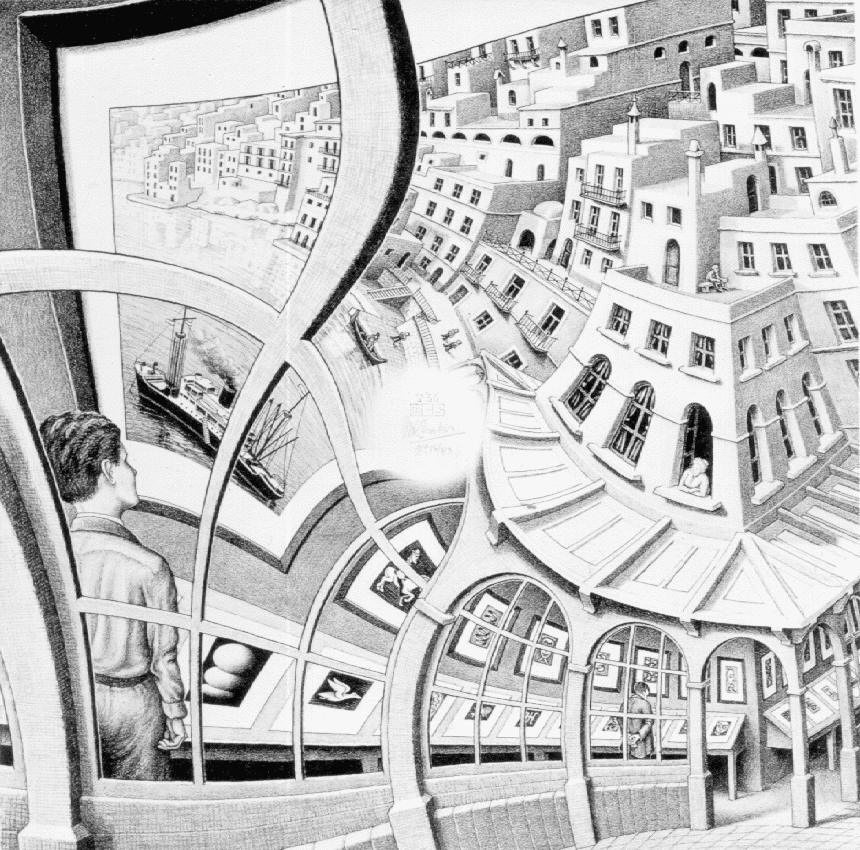
\includegraphics[width=0.5\columnwidth]{GalleriaStampe} 
%\caption[An example of a floating figure]{An example of a floating figure (a reproduction from the \emph{Gallery of prints}, M.~Escher,\index{Escher, M.~C.} from \url{http://www.mcescher.com/}).} % The text in the square bracket is the caption for the list of figures while the text in the curly brackets is the figure caption
%\label{fig:gallery} 
%\end{figure}
%
%\lipsum[5] % Dummy text
%
%\begin{enumerate}[noitemsep] % [noitemsep] removes whitespace between the items for a compact look
%\item First item in a list
%\item Second item in a list
%\item Third item in a list
%\end{enumerate}
%
%%------------------------------------------------
%
%\subsection{Impressionism}

%\lipsum[6] % Dummy text
%
%\paragraph{Paragraph Description} \lipsum[7] % Dummy text
%
%\paragraph{Different Paragraph Description} \lipsum[8] % Dummy text

%------------------------------------------------

\subsection{Important Impressionist Artists in Orsay}
Musee d'Orsay is hosting very important impressionist artists in the world. In this section, most famous ones are listed with brief information.

\subsubsection{Claude Monet}
\begin{figure}[tbH]
\centering
{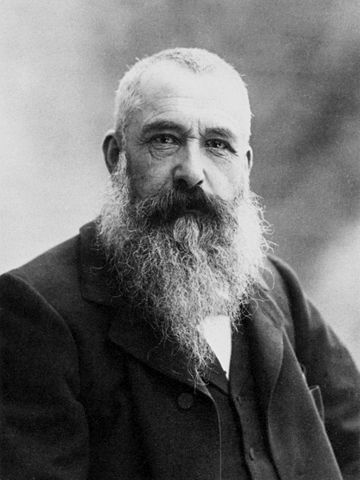
\includegraphics[width=.30\columnwidth]{Images/10.png}}
\caption[Claude Monet]{Claude Monet} % The text in the square bracket is the caption for the list of figures while the text in the curly brackets is the figure caption
\label{fig:claudeMonet}
\end{figure}
\paragraph{}

\paragraph{}
Monet was the founder of French Impressionist, and the most consistent practitioner of the movement. It's said that 'Impressionism' term is coming from his painting 'Impression, soleil levant'. Orsay has his 86 paintings, including The Saint-Lazare Station, The Rue Montorgueil in Paris.

\subsubsection{Vincent van Gogh}
\begin{figure}[tbH]
\centering
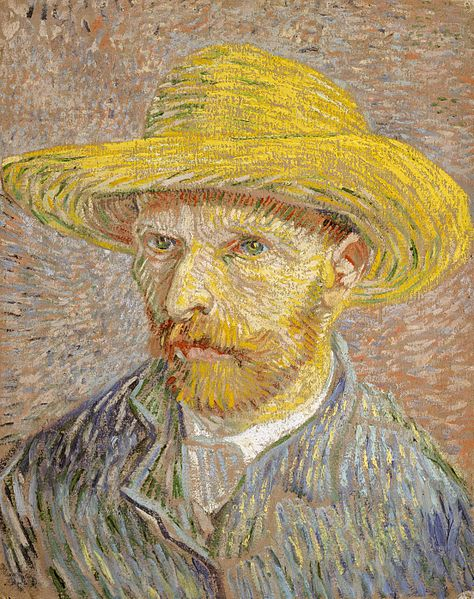
\includegraphics[width=.30\columnwidth]{Images/9.png}
\caption[Vincent van Gogh]{Vincent van Gogh} % The text in the square bracket is the caption for the list of figures while the text in the curly brackets is the figure caption
\label{fig:vanGogh}
\end{figure}

\paragraph{}
He born in 30 March, was a post-impressionist painter. His influence had big impact on 20th century art with his rough beauty, bold color and emotional honesty.  The museum has his 24 works including Self Portrait, portrait of his friend Eugene Boch, The Siesta and many more famous portrait.

\subsubsection{Édouard Manet}
\begin{figure}[tbH]
\centering
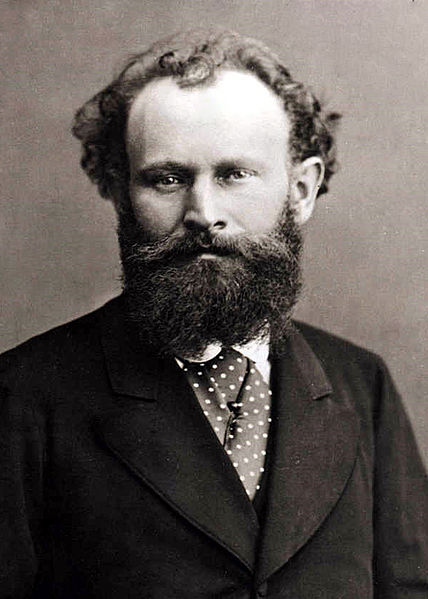
\includegraphics[width=.30\columnwidth]{Images/11.png}
\caption[Édouard Manet]{Édouard Manet} % The text in the square bracket is the caption for the list of figures while the text in the curly brackets is the figure caption
\label{fig:manet}
\end{figure}

\paragraph{}
He was a French paintern born in 23 January, 1832 and one of the first 19th century artists to paint modern life and important figure in transition from Realism to Impressionism. Orsay museum has 34 paintings of him including Olympia, The Balcony, Berthe Morisot With a Bouquet of Violets, The Luncheon on the Grass.

\subsubsection{Edgar Degas}
\begin{figure}[tbH]
\centering
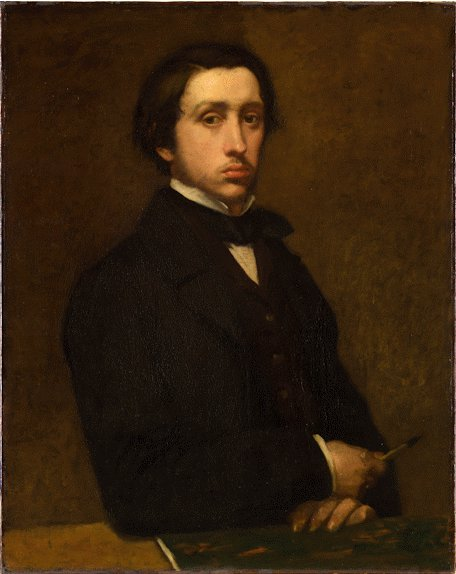
\includegraphics[width=.30\columnwidth]{Images/12.png}
\caption[Edgar Degas]{Edgar Degas} % The text in the square bracket is the caption for the list of figures while the text in the curly brackets is the figure caption
\label{fig:degas}
\end{figure}

\paragraph{}
He, born in 19 July, 1834, was a famous French artist with his paintings, sculptures, prints and drawings. He can be identified with the subject of dance because half of his works showing dancers. He is also regarded as one of the founders of Impressionism. The museum has 43 paintings of him including The Parade, also known as Race Horses in fron of the Tribunes, The Belleli Family, The Tub, Portrait of Eduard Manet and more.

\subsubsection{Pierre-Auguste Renoir}
\begin{figure}[tbH]
\centering
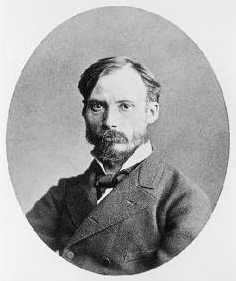
\includegraphics[width=.30\columnwidth]{Images/13.png}
\caption[Pierre-Auguste Renoir]{Pierre-Auguste Renoir} % The text in the square bracket is the caption for the list of figures while the text in the curly brackets is the figure caption
\label{fig:renoir}
\end{figure}

\paragraph{}
One of the French leading painter in the development of the Impressionst style, born in 25 February, 1841. As a celebrator of beauty, and especially feminine sensuality, it has been said that 'Renoir is the final representative of a tradition which runs directly from Rubens to Watteau'. Orsay museum has his 81 paintings including Bal au moulin de la Galette, Montmarte.

\subsubsection{Paul Cézanne}
\begin{figure}[tbH]
\centering
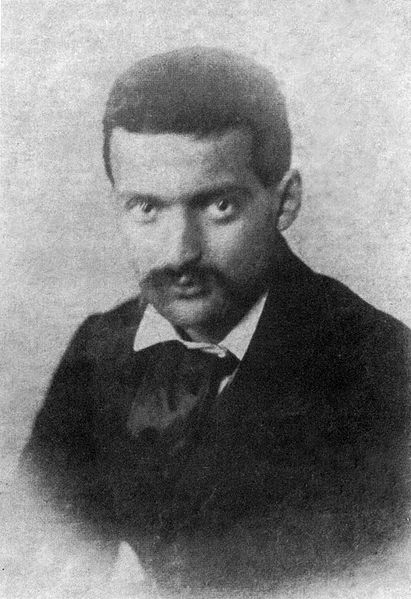
\includegraphics[width=.30\columnwidth]{Images/14.png}
\caption[Paul Cézanne]{Paul Cézanne} % The text in the square bracket is the caption for the list of figures while the text in the curly brackets is the figure caption
\label{fig:cezanne}
\end{figure}

\paragraph{}
Born in 19 January, 1839, he was a French artist and Post-Impressionist painter whose work laid the foundations  of the transition from the 19th century conception of artistic achievement to a new and radically different world of art in the 20th century. The museum has his 56 paintings including Apples and Oranges.

\subsubsection{Georges Seurat}
\begin{figure}[tbH]
\centering
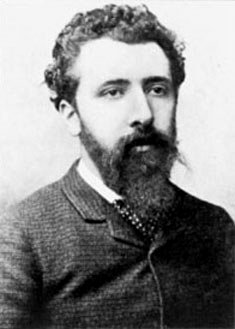
\includegraphics[width=.30\columnwidth]{Images/17.jpg}
\caption[Georges Seurat]{Georges Seurat} % The text in the square bracket is the caption for the list of figures while the text in the curly brackets is the figure caption
\label{fig:seurat}
\end{figure}

\paragraph{}
He was a French Post-Impressionist painter and draftsman. He born in 2 December, 1859. He is known with his innovative use of drawing media and for devising the technique of painting known as pointillism. Orsay museum has his 19 paintings including The Circus.


\subsubsection{Alfred Sisley}
\begin{figure}[tbH]
\centering
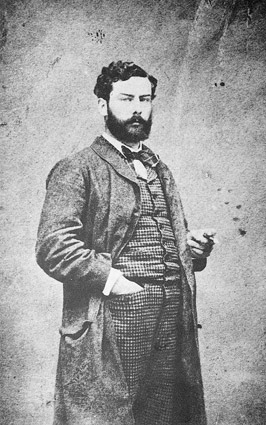
\includegraphics[width=.30\columnwidth]{Images/15.png}
\caption[Alfred Sisley]{Alfred Sisley} % The text in the square bracket is the caption for the list of figures while the text in the curly brackets is the figure caption
\label{fig:sisley}
\end{figure}

\paragraph{}
French painter born in 30 October, 1839. He was an Impressionist landspace painter who was born and spent most of his life in France. He was one of the most consistent of the Impressionists in his dedication to painting landscapes. The museum has his 46 paintings including Inondation at Port-Marly.


\subsubsection{Paul Gauguin}
\begin{figure}[tbH]
\centering
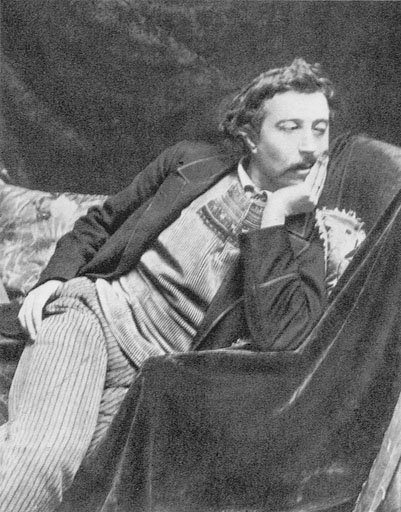
\includegraphics[width=.30\columnwidth]{Images/16.png}
\caption[Paul Gauguin]{Paul Gauguin} % The text in the square bracket is the caption for the list of figures while the text in the curly brackets is the figure caption
\label{fig:gauguin}
\end{figure}

\paragraph{}
Born in 7June, 1848, he is another leading French Post-Impressionist artist who was not well appreciated until his death. Gauguin was later recognized for his experimental use of colors and synthetic style that were distinguishable different from Impressionism. Orsay museum has his 24 paintings including Tahitian Women on the Beach.

%----------------------------------------------------------------------------------------
%	RESULTS AND DISCUSSION
%----------------------------------------------------------------------------------------

\section{Artworks in the Museum}
In this section artworks are picked from famous artists to demonstrate brief collection of the Museum and its important masterpieces. Museum has many different type of art works. Here are some of them.

%------------------------------------------------

\subsection{Paintings}
You can see the famous paintings in Figure~\vref{fig:paintingsFigure}

\begin{figure}[htb]
\centering
\subfloat[Poppy Field]{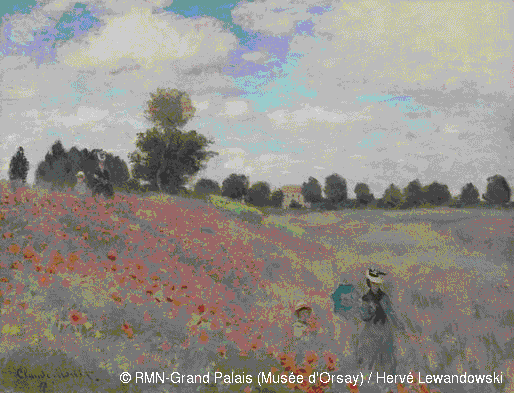
\includegraphics[width=.30\columnwidth]{Images/Paintings/monetPoppyField.png}} \quad
\subfloat[Van Gogh's Bedroom in Arles]{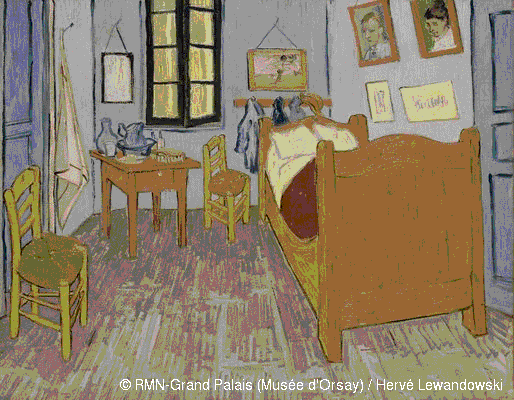
\includegraphics[width=.30\columnwidth]{Images/Paintings/goghBedroom.png}\label{fig:ipsum}} \\ 
\subfloat[Olympia]{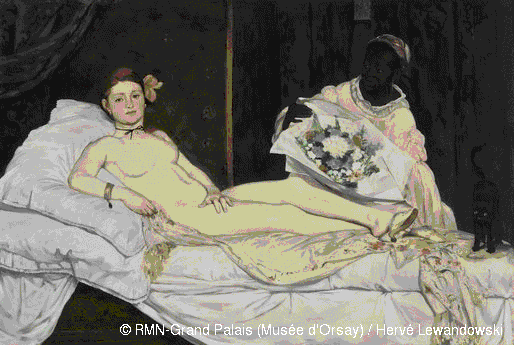
\includegraphics[width=.30\columnwidth]{Images/Paintings/manetOlympia.png}} \quad
\subfloat[Thérèse de Gas]{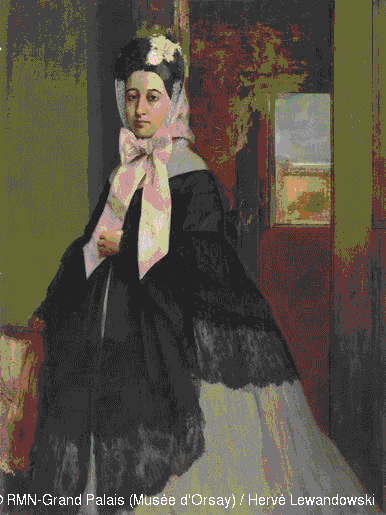
\includegraphics[width=.30\columnwidth]{Images/Paintings/degasGas.png}} \\
\subfloat[The Swing]{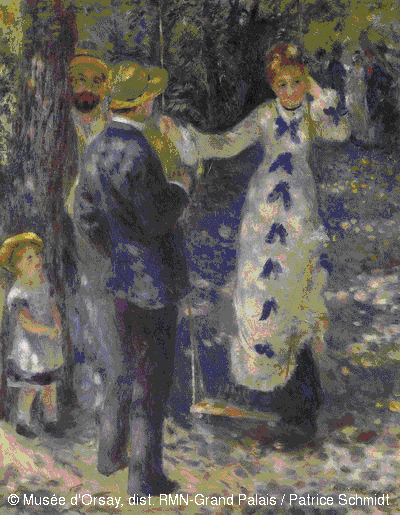
\includegraphics[width=.30\columnwidth]{Images/Paintings/renoirSwing.png}} \quad
\subfloat[The Bay of Marseille seen from L'Estaque]{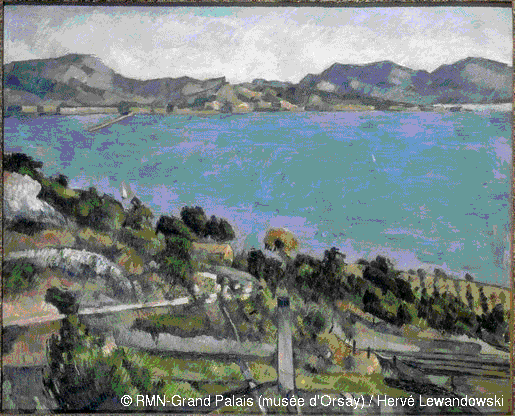
\includegraphics[width=.30\columnwidth]{Images/Paintings/cezanneMarseille.png}\label{fig:ipsum}} \\ \pagebreak
\subfloat[Port-en-Bessin at High Tide]{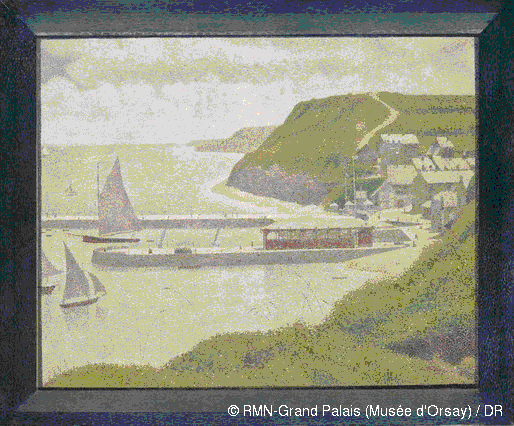
\includegraphics[width=.30\columnwidth]{Images/Paintings/seuratPort.png}} \quad
\subfloat[Fog, Voisins]{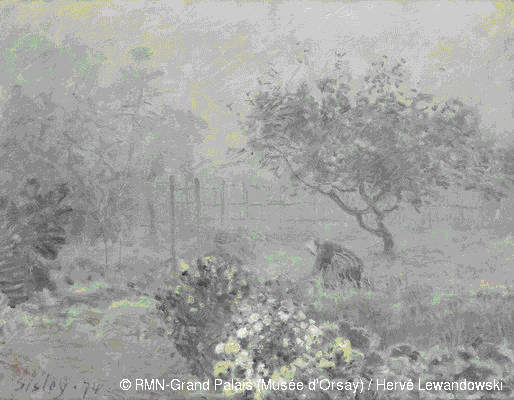
\includegraphics[width=.30\columnwidth]{Images/Paintings/sisleyFog.png}} \\
\subfloat[Les Alyscamps]{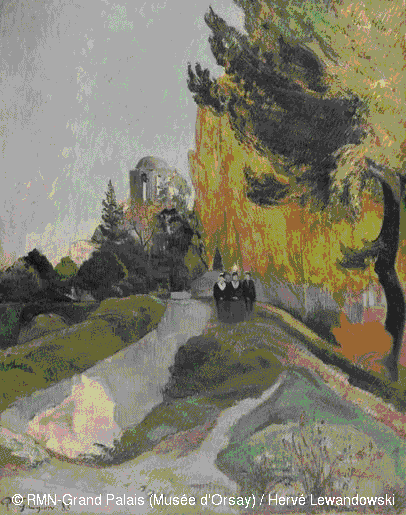
\includegraphics[width=.30\columnwidth]{Images/Paintings/gauguinAlyscamps.png}} 


\caption[A number of pictures of impressionist artists ]{A number of pictures of impressionist artists} % The text in the square bracket is the caption for the list of figures while the text in the curly brackets is the figure caption
\label{fig:paintingsFigure}
\end{figure}

\subsection{Sculptures}

\subsection{Photography}

\subsection{Graphic Art}

\subsection{Decoratives}

\subsection{Architecture}

%\lipsum[12] % Dummy text
%
%\begin{description}
%\item[Word] Definition
%\item[Concept] Explanation
%\item[Idea] Text
%\end{description}
%
%\lipsum[12] % Dummy text
%
%\begin{itemize}[noitemsep] % [noitemsep] removes whitespace between the items for a compact look
%\item First item in a list
%\item Second item in a list
%\item Third item in a list
%\end{itemize}
%
%\subsubsection{Table}
%
%\lipsum[13] % Dummy text
%
%\begin{table}[hbt]
%\caption{Table of Grades}
%\centering
%\begin{tabular}{llr}
%\toprule
%\multicolumn{2}{c}{Name} \\
%\cmidrule(r){1-2}
%First name & Last Name & Grade \\
%\midrule
%John & Doe & $7.5$ \\
%Richard & Miles & $2$ \\
%\bottomrule
%\end{tabular}
%\label{tab:label}
%\end{table}
%
%Reference to Table~\vref{tab:label}. % The \vref command specifies the location of the reference
%
%%------------------------------------------------
%
%\subsection{Figure Composed of Subfigures}
%
%Reference the figure composed of multiple subfigures as Figure~\vref{fig:esempio}. Reference one of the subfigures as Figure~\vref{fig:ipsum}. % The \vref command specifies the location of the reference
%
%\lipsum[15-18] % Dummy text
%
%\begin{figure}[tbh]
%\centering
%\subfloat[A city market.]{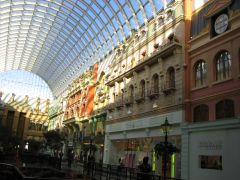
\includegraphics[width=.45\columnwidth]{Lorem}} \quad
%\subfloat[Forest landscape.]{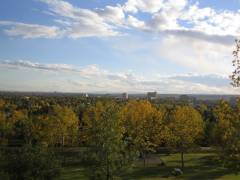
\includegraphics[width=.45\columnwidth]{Ipsum}\label{fig:ipsum}} \\
%\subfloat[Mountain landscape.]{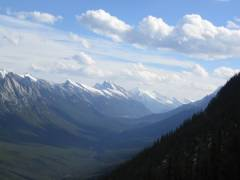
\includegraphics[width=.45\columnwidth]{Dolor}} \quad
%\subfloat[A tile decoration.]{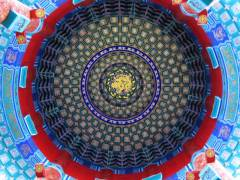
\includegraphics[width=.45\columnwidth]{Sit}}
%\caption[A number of pictures.]{A number of pictures with no common theme.} % The text in the square bracket is the caption for the list of figures while the text in the curly brackets is the figure caption
%\label{fig:esempio}
%\end{figure}

%----------------------------------------------------------------------------------------
%	BIBLIOGRAPHY
%----------------------------------------------------------------------------------------

\renewcommand{\refname}{\spacedlowsmallcaps{References}} % For modifying the bibliography heading

%\bibliographystyle{unsrt}

%----------------------------------------------------------------------------------------

\begin{thebibliography}{10}

 \bibitem{wikipediaOrsay} Wikipedia {\em Musée d'Orsay}  2014: \url{http://en.wikipedia.org/wiki/Mus\%C3\%A9e_d'Orsay}.
 
 \bibitem{orsayMuseumHistory} Musée d'Orsay {\em History of the museum}  2014: \url{http://www.musee-orsay.fr/en/collections/history-of-the-museum/home.html}.
 
\bibitem{wikipediaImpressionism} Wikipedia {\em Impressionism}  2014: \url{http://en.wikipedia.org/wiki/Impressionism}.

\bibitem{wikipediaImpressionism} Wikipedia {\em Claude Monet}  2014: \url{http://en.wikipedia.org/wiki/Monet}.

\bibitem{wikipediaImpressionism} Wikipedia {\em Vincent van Gogh}  2014: \url{http://en.wikipedia.org/wiki/Van_Gogh}.

\bibitem{wikipediaImpressionism} Wikipedia {\em Édouard Manet}  2014: \url{http://en.wikipedia.org/wiki/Manet}.

\bibitem{wikipediaImpressionism} Wikipedia {\em Edgar Degas}  2014: \url{http://en.wikipedia.org/wiki/Degas}.

\bibitem{wikipediaImpressionism} Wikipedia {\em Pierre-Auguste Renoir}  2014: \url{http://en.wikipedia.org/wiki/Renoir}.

\bibitem{wikipediaImpressionism} Wikipedia {\em Paul Cézanne}  2014: \url{http://en.wikipedia.org/wiki/C%C3%A9zanne}.

\bibitem{wikipediaImpressionism} Wikipedia {\em Georges Seurat}  2014: \url{http://en.wikipedia.org/wiki/Seurat}.

\bibitem{wikipediaImpressionism} Wikipedia {\em Alfred Sisley}  2014: \url{http://en.wikipedia.org/wiki/Alfred_Sisley}.

\bibitem{wikipediaImpressionism} Wikipedia {\em Paul Gauguin}  2014: \url{http://en.wikipedia.org/wiki/Gauguin}.


\end{thebibliography}

\end{document}